
%  Multigrid FSP for the RDME — v4
%  Aditya Dendukuri

\documentclass[10pt,aspectratio=169]{beamer}

\usetheme{Boadilla}
\usecolortheme{seahorse}
\setbeamertemplate{navigation symbols}{}
\setbeamerfont{frametitle}{size=\normalsize,series=\bfseries}
\setbeamerfont{title}{size=\large,series=\bfseries}
\setbeamertemplate{bibliography item}[text]

\usepackage{amsmath,amssymb,bm,mathtools}
\usepackage{tikz}
\usetikzlibrary{arrows.meta,positioning,patterns,decorations.pathreplacing,calc}
\usepackage{graphicx}
\usepackage{booktabs}
\usepackage{xcolor}
\usepackage{colortbl}
\usepackage{pifont}

\graphicspath{{figures/}}

\newcommand{\Bin}{\operatorname{Bin}}
\newcommand{\Mult}{\operatorname{Mult}}
\newcommand{\calR}{\mathcal{R}}
\newcommand{\calP}{\mathcal{P}}
\newcommand{\citeref}[1]{{\scriptsize\textcolor{gray}{[#1]}}}

\definecolor{fastblue}{RGB}{31,119,180}
\definecolor{slowred}{RGB}{214,39,40}
\definecolor{coarsegreen}{RGB}{44,160,44}
\definecolor{coarsecolor}{RGB}{31,119,180}
\definecolor{intercolor}{RGB}{255,140,0}
\definecolor{myblue}{RGB}{31,119,180}
\definecolor{mygray}{RGB}{80,80,80}
\definecolor{activegreen}{RGB}{44,160,44}
\definecolor{mfgray}{RGB}{150,150,150}

\title[Multigrid FSP for RDME]{%
  Multigrid Finite State Projection\\
  for the Reaction-Diffusion Master Equation}
\author{Aditya Dendukuri}
\institute[UCSB]{University of California, Santa Barbara}
\date{}

\begin{document}

\begin{frame}\titlepage\end{frame}


% ================================================================
%  1. RDME intro
% ================================================================
\begin{frame}{The RDME: reactions and diffusion across a spatial grid}

  \begin{columns}[T]
    \begin{column}{0.50\textwidth}
      \textbf{Model.}
      Divide a 1-D domain into $K$ voxels.
      Each voxel $k$ holds molecule counts $\mathbf{n}_k \in \mathbb{Z}_{\geq 0}^S$.

      \medskip
      Two types of events:
      \begin{itemize}\setlength\itemsep{0.4em}
        \item \textcolor{slowred}{\textbf{Reactions}} inside voxel $k$:
              rate $\alpha_r(\mathbf{n}_k)$, change $\mathbf{n}_k$.
        \item \textcolor{fastblue}{\textbf{Diffusion}} between neighbors:
              rate $d = D/h^2$, moves one molecule $k \leftrightarrow k{+}1$.
      \end{itemize}

      \medskip
      The joint probability $p(\mathbf{n}_1,\ldots,\mathbf{n}_K,t)$
      satisfies $\dot p = A p$ \textbf{(RDME)}.

      \medskip
      \begin{alertblock}{The computational bottleneck}
        The state space has $\sim n_{\max}^{SK}$ reachable states ---
        \textbf{exponential in $K$}.
        Even $K{=}8$, $S{=}1$ is intractable with a naive FSP.
      \end{alertblock}
    \end{column}
    \begin{column}{0.46\textwidth}
      \begin{center}
      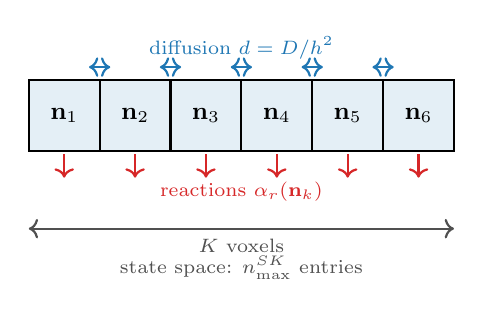
\begin{tikzpicture}[scale=0.90, every node/.style={font=\small}]
        \foreach \k in {1,2,3,4,5,6} {
          \draw[thick,fill=myblue!12] (\k-1,0) rectangle (\k,1.0);
          \node at (\k-0.5, 0.50) {$\mathbf{n}_\k$};
        }
        \foreach \k in {1,2,3,4,5} {
          \draw[<->,fastblue,thick] (\k-0.15,1.18) -- (\k+0.15,1.18);
        }
        \node[fastblue, font=\scriptsize] at (3, 1.45) {diffusion $d = D/h^2$};
        \foreach \k in {1,2,3,4,5,6} {
          \draw[->,slowred,thick] (\k-0.5,-0.05) -- (\k-0.5,-0.38);
        }
        \node[slowred, font=\scriptsize] at (3, -0.58) {reactions $\alpha_r(\mathbf{n}_k)$};
        \draw[<->,thick,mygray] (0,-1.1) -- (6,-1.1)
          node[midway,below,font=\scriptsize]{$K$ voxels};
        \node[mygray,font=\scriptsize] at (3,-1.65)
          {state space: $n_{\max}^{SK}$ entries};
      \end{tikzpicture}
      \end{center}
    \end{column}
  \end{columns}

\end{frame}


% ================================================================
%  2. Block-tridiagonal structure
% ================================================================
\begin{frame}{$\dot{p} = Ap$ has block-tridiagonal structure \textnormal{\small(schematic, $K{=}4$, $S{=}1$)}}

\vspace{-0.2cm}
\begin{center}
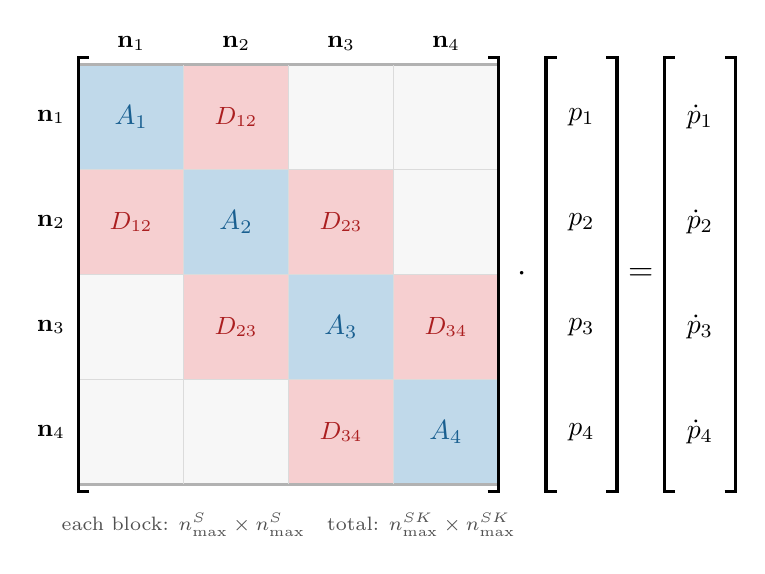
\begin{tikzpicture}[scale=0.86]
  \def\bs{1.55}
  \def\bw{0.16}
  \def\bp{0.10}

  \fill[gray!6] (0,0) rectangle (4*\bs,4*\bs);
  \foreach \k in {0,1,2,3}
    \fill[myblue!28] (\k*\bs,{(3-\k)*\bs}) rectangle ({(\k+1)*\bs},{(4-\k)*\bs});
  \foreach \k in {0,1,2} {
    \fill[slowred!22] ({(\k+1)*\bs},{(3-\k)*\bs}) rectangle ({(\k+2)*\bs},{(4-\k)*\bs});
    \fill[slowred!22] ({\k*\bs},{(2-\k)*\bs}) rectangle ({(\k+1)*\bs},{(3-\k)*\bs});
  }
  \draw[black!30,thick] (0,0) rectangle (4*\bs,4*\bs);
  \foreach \k in {1,2,3} {
    \draw[black!14,thin] (\k*\bs,0) -- (\k*\bs,4*\bs);
    \draw[black!14,thin] (0,\k*\bs) -- (4*\bs,\k*\bs);
  }
  \foreach \k/\l in {0/1,1/2,2/3,3/4}
    \node[font=\normalsize, myblue!80!black]
      at ({(\k+0.5)*\bs},{(3.5-\k)*\bs}) {$A_\l$};
  \node[font=\small,slowred!80!black] at (1.5*\bs,3.5*\bs) {$D_{12}$};
  \node[font=\small,slowred!80!black] at (0.5*\bs,2.5*\bs) {$D_{12}$};
  \node[font=\small,slowred!80!black] at (2.5*\bs,2.5*\bs) {$D_{23}$};
  \node[font=\small,slowred!80!black] at (1.5*\bs,1.5*\bs) {$D_{23}$};
  \node[font=\small,slowred!80!black] at (3.5*\bs,1.5*\bs) {$D_{34}$};
  \node[font=\small,slowred!80!black] at (2.5*\bs,0.5*\bs) {$D_{34}$};
  \foreach \k/\l in {0/$\mathbf{n}_1$,1/$\mathbf{n}_2$,2/$\mathbf{n}_3$,3/$\mathbf{n}_4$} {
    \node[above,font=\small] at ({(\k+0.5)*\bs}, 4*\bs+0.06) {\l};
    \node[left, font=\small] at (-0.06, {(3.5-\k)*\bs}) {\l};
  }
  \draw[very thick]
    (\bw,-\bp) -- (0,-\bp) -- (0,4*\bs+\bp) -- (\bw,4*\bs+\bp);
  \draw[very thick]
    (4*\bs-\bw,-\bp) -- (4*\bs,-\bp) -- (4*\bs,4*\bs+\bp) -- (4*\bs-\bw,4*\bs+\bp);
  \def\vgap{0.70}
  \def\vw{1.05}
  \pgfmathsetmacro{\vx}{4*\bs + \vgap}
  \node[font=\large] at ({4*\bs + \vgap/2}, {2*\bs}) {$\cdot$};
  \draw[very thick]
    (\vx+\bw,-\bp) -- (\vx,-\bp) -- (\vx,4*\bs+\bp) -- (\vx+\bw,4*\bs+\bp);
  \draw[very thick]
    (\vx+\vw-\bw,-\bp) -- (\vx+\vw,-\bp) -- (\vx+\vw,4*\bs+\bp)
    -- (\vx+\vw-\bw,4*\bs+\bp);
  \foreach \k/\l in {0/$p_1$,1/$p_2$,2/$p_3$,3/$p_4$}
    \node[font=\normalsize] at (\vx+\vw/2, {(3.5-\k)*\bs}) {\l};
  \pgfmathsetmacro{\eqx}{\vx + \vw + \vgap/2}
  \node[font=\large] at (\eqx, {2*\bs}) {$=$};
  \pgfmathsetmacro{\rx}{\vx + \vw + \vgap}
  \draw[very thick]
    (\rx+\bw,-\bp) -- (\rx,-\bp) -- (\rx,4*\bs+\bp) -- (\rx+\bw,4*\bs+\bp);
  \draw[very thick]
    (\rx+\vw-\bw,-\bp) -- (\rx+\vw,-\bp) -- (\rx+\vw,4*\bs+\bp)
    -- (\rx+\vw-\bw,4*\bs+\bp);
  \foreach \k/\l in {0/$\dot p_1$,1/$\dot p_2$,2/$\dot p_3$,3/$\dot p_4$}
    \node[font=\normalsize] at (\rx+\vw/2, {(3.5-\k)*\bs}) {\l};
  \node[mygray,font=\scriptsize,below] at (2*\bs,-\bp-0.18)
    {each block: $n_{\max}^S \times n_{\max}^S$\quad total: $n_{\max}^{SK} \times n_{\max}^{SK}$};
\end{tikzpicture}
\end{center}

\vspace{0.2em}
{\small
  \textcolor{myblue!80!black}{$A_k$}: reactions inside voxel $k$ (dense block)
  \hspace{1.5em}
  \textcolor{slowred!80!black}{$D_{k,k+1}$}: diffusion between neighboring voxels (sparse: shifts one count)\\[0.3em]
  \textbf{Key structure:} diffusion only couples \emph{adjacent} blocks.
  This locality is what makes spatial coarsening (merging adjacent blocks) exact.
}

\end{frame}


% ================================================================
%  3. Binomial equilibrium
% ================================================================
\begin{frame}{The Binomial is the exact diffusion equilibrium}

  \begin{columns}[T]
    \begin{column}{0.50\textwidth}
      \textbf{Fix total molecules} $\bar n = n_1 + n_2$ across two adjacent voxels.

      \smallskip
      Diffusion moves one molecule at a time, at rate $d$ per molecule:

      \begin{center}
      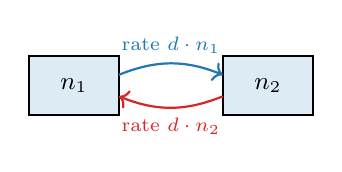
\begin{tikzpicture}[every node/.style={font=\small}, scale=0.88]
        \draw[thick,fill=coarsecolor!15] (0,0) rectangle (1.3,0.85);
        \draw[thick,fill=coarsecolor!15] (2.8,0) rectangle (4.1,0.85);
        \node at (0.65, 0.42) {$n_1$};
        \node at (3.45, 0.42) {$n_2$};
        \draw[->,fastblue,thick,bend left=22] (1.3,0.58)
          to node[above,font=\scriptsize]{rate $d\cdot n_1$} (2.8,0.58);
        \draw[->,slowred,thick,bend left=22]  (2.8,0.27)
          to node[below,font=\scriptsize]{rate $d\cdot n_2$} (1.3,0.27);
      \end{tikzpicture}
      \end{center}

      Each molecule hops independently $\Rightarrow$ at equilibrium, equally
      likely to be in either voxel. For $\bar n$ total:
      \[
        \boxed{P(n_1 \mid \bar n) = \Bin\!\bigl(\bar n,\,\tfrac{1}{2}\bigr)}
        \quad \text{(exact, any } d > 0\text{)}
      \]
      When the distribution is near this equilibrium,
      \textbf{$\bar n$ alone describes the two-voxel state}.
    \end{column}
    \begin{column}{0.46\textwidth}
      \begin{center}
      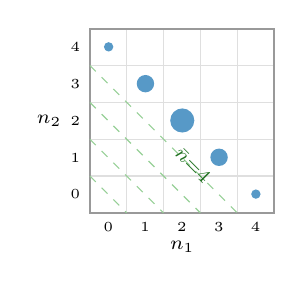
\begin{tikzpicture}[scale=0.85]
        \def\cs{0.55}
        \draw[gray!25](0,0) grid[step=\cs] (5*\cs,5*\cs);
        \draw[black!40,thick](0,0) rectangle (5*\cs,5*\cs);
        \foreach \t in {1,2,3,4} {
          \draw[coarsegreen!50,dashed,thin]
            ({max(0,\t-4)*\cs},{min(\t,4)*\cs}) -- ({min(\t,4)*\cs},{max(0,\t-4)*\cs});
        }
        \fill[coarsecolor!75](0.28,2.48) circle (0.07cm);
        \fill[coarsecolor!75](0.83,1.93) circle (0.13cm);
        \fill[coarsecolor!75](1.38,1.38) circle (0.18cm);
        \fill[coarsecolor!75](1.93,0.83) circle (0.13cm);
        \fill[coarsecolor!75](2.48,0.28) circle (0.07cm);
        \foreach \n in {0,1,2,3,4}
          \node[below,font=\tiny] at ({(\n+0.5)*\cs},0) {\n};
        \foreach \n in {0,1,2,3,4}
          \node[left,font=\tiny]  at (0,{(\n+0.5)*\cs}) {\n};
        \node[below,font=\scriptsize] at (1.38,-0.28) {$n_1$};
        \node[left, font=\scriptsize] at (-0.28,1.38) {$n_2$};
        \node[coarsegreen!70!black,font=\scriptsize,rotate=-45] at (2.8*\cs,1.3*\cs) {$\bar n{=}4$};
      \end{tikzpicture}

      \vspace{0.4em}
      {\footnotesize
        Probability spreads along constant-total diagonals
        as $\Bin(\bar n,\tfrac12)$ (dot size $\propto$ mass).\\[0.3em]
        \textbf{The two-voxel state is captured by $\bar n$ alone.}
      }
      \end{center}
    \end{column}
  \end{columns}

\end{frame}


% ================================================================
%  3. Restriction and prolongation
% ================================================================
\begin{frame}{Merging two adjacent voxels: restriction and prolongation}

  \begin{columns}[T]
    \begin{column}{0.50\textwidth}
      \textbf{Compress ($\calR$): exact:}
      \[ p^c(\bar n) = \!\!\sum_{n_1 + n_2 = \bar n}\!\! p(n_1, n_2). \]

      \textbf{Reconstruct ($\calP$): approximate:}
      \[ p(n_1, n_2) \approx p^c(\bar n)\cdot\pi(\bar n), \]
      where $\pi$ is the \textbf{within-pair distribution}.

      \begin{block}{State-space reduction}
        Per pair: $n_{\max}^{2S} \to n_{\max}^{S}$.\\
        All $K$ voxels: $n_{\max}^{SK} \to n_{\max}^{SK/2}$.
      \end{block}

      \smallskip
      {\small
        Classical choice: $\pi = \Bin(\bar n,\tfrac12)$ --- exact when
        diffusion $\gg$ reactions.\\[0.3em]
        \textbf{New:} patch QSD (later) --- exact conditional distribution
        accounting for reactions within the patch.
      }
    \end{column}
    \begin{column}{0.46\textwidth}
      \begin{center}
      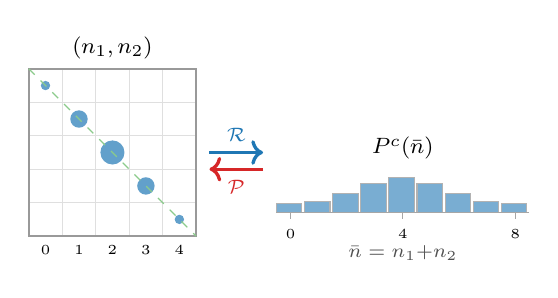
\begin{tikzpicture}[scale=0.85, every node/.style={font=\scriptsize}]
        \def\cs{0.50}
        \draw[gray!25](0,0) grid[step=\cs] (5*\cs,5*\cs);
        \draw[black!40,thick](0,0) rectangle (5*\cs,5*\cs);
        \node[above,font=\footnotesize] at (1.25,2.5) {$(n_1,n_2)$};
        \fill[coarsecolor!70](0.25,2.25) circle (0.07cm);
        \fill[coarsecolor!70](0.75,1.75) circle (0.13cm);
        \fill[coarsecolor!70](1.25,1.25) circle (0.18cm);
        \fill[coarsecolor!70](1.75,0.75) circle (0.13cm);
        \fill[coarsecolor!70](2.25,0.25) circle (0.07cm);
        \draw[coarsegreen!55,dashed](0,2.5)--(2.5,0);
        \foreach \n in {0,1,2,3,4}
          \node[below,font=\tiny] at ({(\n+0.5)*\cs},0) {\n};
        \draw[->,very thick,coarsecolor] (2.7,1.25) -- (3.5,1.25)
          node[above,midway,font=\scriptsize]{$\calR$};
        \draw[->,very thick,slowred]     (3.5,1.0)  -- (2.7,1.0)
          node[below,midway,font=\scriptsize]{$\calP$};
        \def\cb{0.42}
        \foreach \nb in {0,1,2,3,4,5,6,7,8} {
          \pgfmathsetmacro{\ht}{0.12 + 0.40*exp(-0.5*((\nb-4)/1.5)*((\nb-4)/1.5))}
          \fill[coarsecolor!60] (3.7+\nb*\cb, 0.35) rectangle
                                (3.7+\nb*\cb+\cb-0.04, 0.35+\ht);
          \draw[black!30] (3.7+\nb*\cb, 0.35) rectangle
                          (3.7+\nb*\cb+\cb-0.04, 0.35+\ht);
        }
        \draw[black!35] (3.7,0.35) -- (3.7+9*\cb,0.35);
        \foreach \nb/\lbl in {0/0, 4/4, 8/8} {
          \draw[black!35] (3.7+\nb*\cb+\cb/2,0.35) -- (3.7+\nb*\cb+\cb/2,0.25);
          \node[below,font=\tiny] at (3.7+\nb*\cb+\cb/2,0.25) {\lbl};
        }
        \node[below,font=\scriptsize,mygray] at (3.7+4.5*\cb,0.0)
          {$\bar n = n_1{+}n_2$};
        \node[above,font=\footnotesize] at (3.7+4*\cb+\cb/2, 1.0) {$P^c(\bar n)$};
      \end{tikzpicture}

      \vspace{0.3em}
      {\footnotesize
        $\calR$: sum along each diagonal $\to$ scalar $\bar n = n_1{+}n_2$.\\
        $\calP$: spread back via within-pair distribution $\pi$.
      }
      \end{center}
    \end{column}
  \end{columns}

\end{frame}


% ================================================================
%  4. Adaptive FSP
% ================================================================
\begin{frame}{The adaptive FSP algorithm: expand, solve, prune}
\begin{center}
  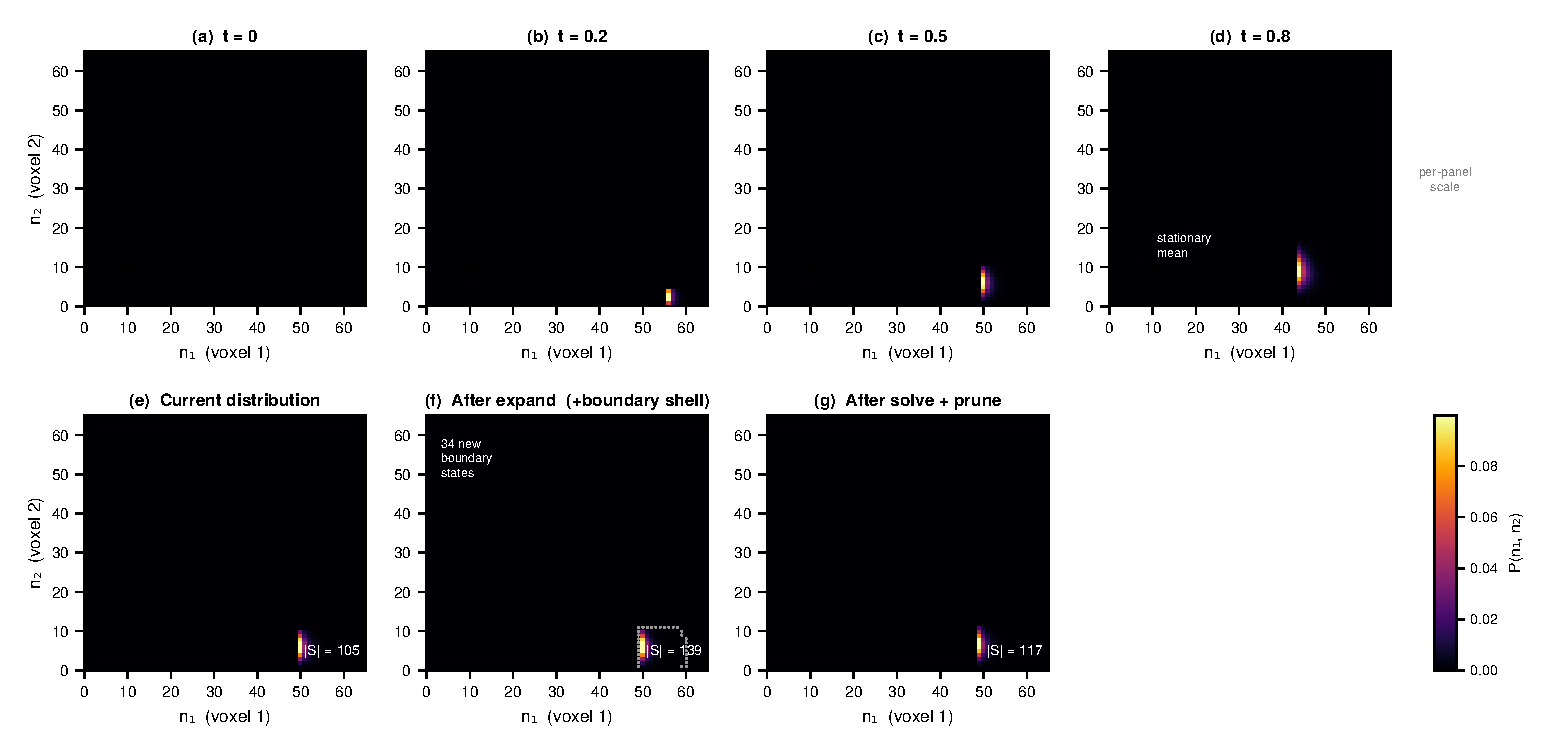
\includegraphics[width=0.92\textwidth,keepaspectratio]{fig_talk_fsp}
\end{center}
\vspace{-0.4em}
{\small
\textbf{Top row:} joint distribution $P(n_1,n_2)$ of a 2-voxel birth-death system: point source at $(n_\text{src},0)$ traveling to the stationary point (white cross).\\[0.2em]
\textbf{Bottom row} (one step at $t{=}0.5$):
\textbf{(e)}~Current support $|S|{=}105$.
\textbf{(f)}~After expand $|S|{=}139$: thin boundary shell added (white dots).
\textbf{(g)}~After solve+prune $|S|{=}117$: compact again.}
\end{frame}


% ================================================================
%  5. Birth-death wavefront result
% ================================================================
\begin{frame}{Result: K=8 RDME wavefront via coarsened simulation}
\begin{center}
  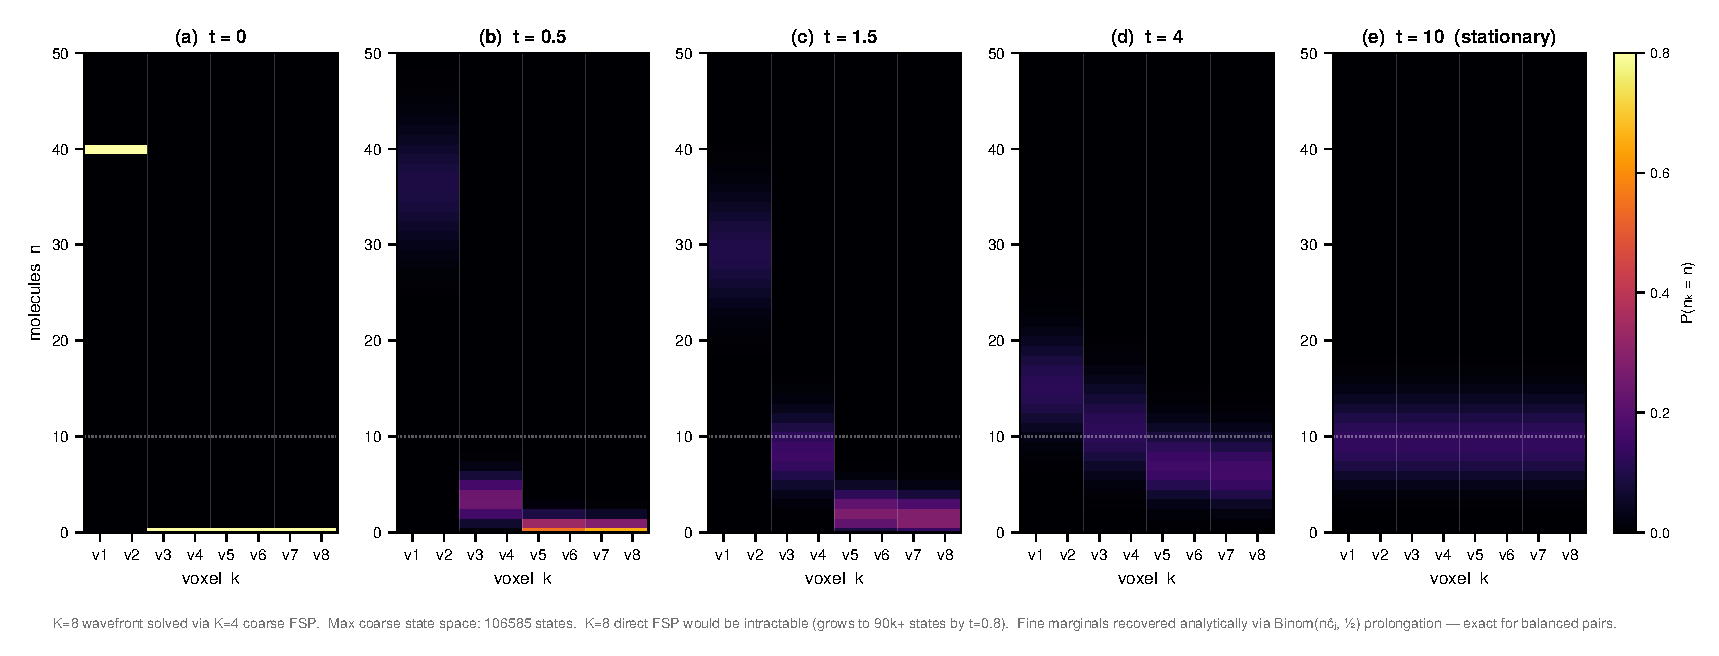
\includegraphics[width=0.92\textwidth,keepaspectratio]{fig_talk_result}
\end{center}
\vspace{-0.4em}
{\small
Birth-death RDME, $K{=}8$, $D{=}0.1$.
IC: $v_1{=}v_2{=}40$ (delta), $v_3\ldots v_8{=}0$.
Each panel shows marginals $P(n_k{=}n)$ for all 8 voxels.\\[0.2em]
\textbf{(a)--(d):} Wavefront sweeps left$\to$right, distributions broaden.
\textbf{(e):} Stationary: all voxels reach $\operatorname{Poisson}(10)$ (dashed line).\\[0.2em]
Solved via \textbf{K=4 coarse FSP} (30k states). Direct K=8 FSP: intractable.
Fine marginals recovered via $\operatorname{Bin}(\tilde{n},\tfrac12)$: exact for balanced pairs.}
\end{frame}


% ================================================================
%  6. NEW: Mixed-resolution active set
% ================================================================
\begin{frame}{Mixed resolution: only the wavefront needs fine tracking}

  \begin{columns}[T]
    \begin{column}{0.52\textwidth}
      \textbf{Key observation:} at any time $t$, the probability distribution
      has \emph{three} spatial zones:

      \medskip
      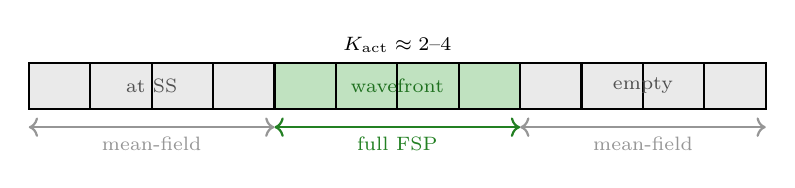
\begin{tikzpicture}[scale=0.78, every node/.style={font=\small}]
        % Full grid
        \foreach \k in {1,...,12} {
          \pgfmathtruncatemacro{\zone}{
            (\k <= 4) ? 1 : ((\k <= 8) ? 2 : 3)}
          \ifnum\zone=1
            \fill[mfgray!20] (\k-1,0) rectangle (\k,0.75);
          \fi
          \ifnum\zone=2
            \fill[activegreen!30] (\k-1,0) rectangle (\k,0.75);
          \fi
          \ifnum\zone=3
            \fill[mfgray!20] (\k-1,0) rectangle (\k,0.75);
          \fi
          \draw[thick] (\k-1,0) rectangle (\k,0.75);
        }
        % Labels
        \node[font=\scriptsize,mygray] at (2, 0.38) {at SS};
        \node[font=\scriptsize,activegreen!70!black] at (6, 0.38) {wavefront};
        \node[font=\scriptsize,mygray] at (10, 0.38) {empty};
        % Arrows
        \draw[<->,mfgray,thick] (0,-0.3) -- (4,-0.3)
          node[midway,below,font=\scriptsize]{mean-field};
        \draw[<->,activegreen!80!black,thick] (4,-0.3) -- (8,-0.3)
          node[midway,below,font=\scriptsize]{full FSP};
        \draw[<->,mfgray,thick] (8,-0.3) -- (12,-0.3)
          node[midway,below,font=\scriptsize]{mean-field};
        \node[above,font=\scriptsize] at (6,0.75) {$K_{\rm act} \approx 2$--$4$};
      \end{tikzpicture}

      \medskip
      \begin{itemize}\setlength\itemsep{0.3em}
        \item \textbf{At steady state} (behind front):
              $P(\mathbf{n}_k)$ is near-Poisson$(\mu_{\rm ss})$
              $\Rightarrow$ mean-field $\mu_k$ is sufficient.
        \item \textbf{Empty} (ahead of front):
              $P(\mathbf{n}_k) \approx \delta_0$
              $\Rightarrow$ mean-field $\mu_k \approx 0$.
        \item \textbf{Wavefront}: full joint FSP on $K_{\rm act}$ voxels.
              $K_{\rm act} \ll K$, \emph{independent of $K$}.
      \end{itemize}

      \begin{block}{State-space bound}
        $|S_{\rm active}| = O\!\left(n_{\max}^{2S K_{\rm act}}\right)$
        regardless of $K$.
      \end{block}
    \end{column}
    \begin{column}{0.44\textwidth}
      \textbf{Adaptive active set:}

      \medskip
      \begin{itemize}\setlength\itemsep{0.25em}
        \item \textbf{Promote} voxel to FSP when $\mu_k > \theta_{\rm promote}$
              (wavefront arriving).
        \item \textbf{Demote} to mean-field when
              $\mu_k \approx \mu_{\rm ss}$ (converged)
              or $\mu_k \approx 0$ (empty).
        \item Mean-field ODE for inactive voxels --- \emph{exact for linear reactions}.
        \item Hard cap $K_{\rm act}^{\max}$ prevents blowup for fast diffusion.
      \end{itemize}

      \medskip
      \begin{center}
      \includegraphics[width=0.98\textwidth,keepaspectratio]{mixed_multigrid_1d}
      \end{center}
      {\scriptsize
        $K{=}32$, $D{=}0.001$: $K_{\rm act}{\leq}4$ throughout (white active window overlaid).
        $|S_{\rm active}|{\leq}5000$; direct K=32 FSP would require ${\sim}10^{32}$ states.
      }
    \end{column}
  \end{columns}

\end{frame}


% ================================================================
%  7. Bistability
% ================================================================
\begin{frame}{Bistable reactions}

\begin{columns}[T]
\column{0.50\textwidth}
For birth-death, each voxel has one stable state.
Diffusion wins: the pair is always well-mixed.
Binomial coarsening is \emph{essentially exact}.

\vspace{0.8em}
\textbf{But what if reactions are bistable?}\\[0.4em]
The \textbf{Schl\"{o}gl model} has two stable states per voxel:
$n_\text{lo} \approx 31$ and $n_\text{hi} \approx 162$.

\vspace{0.4em}
\begin{center}
  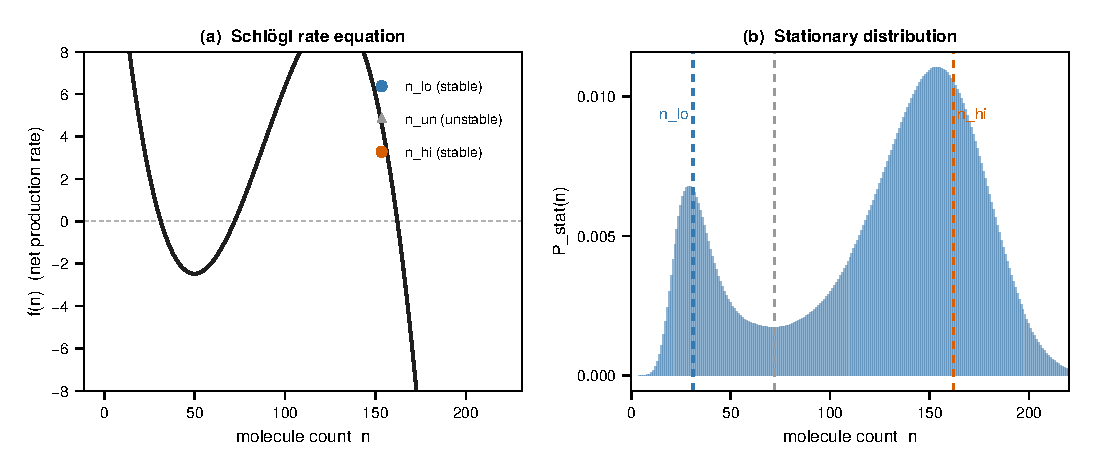
\includegraphics[width=0.95\textwidth]{fig_talk_bistability}
\end{center}

\column{0.46\textwidth}
\vspace{0.3em}
\begin{block}{Spatial metastability}
Neighbors can occupy \emph{different} states.
A \textbf{spatial front} forms.
\end{block}

\medskip
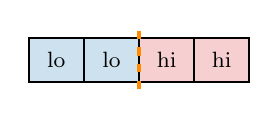
\begin{tikzpicture}[scale=0.7, every node/.style={font=\footnotesize}]
  \foreach \k in {1,2} {
    \draw[thick,fill=myblue!22] (\k-1,0) rectangle (\k,0.8);
    \node at (\k-0.5,0.4) {lo};
  }
  \foreach \k in {3,4} {
    \draw[thick,fill=slowred!22] (\k-1,0) rectangle (\k,0.8);
    \node at (\k-0.5,0.4) {hi};
  }
  \draw[very thick,intercolor,dashed] (2,-0.12) -- (2,0.96);
\end{tikzpicture}

\medskip
{\small Reactions ``pull'' voxels apart; diffusion ``pulls'' them together.
When reactions are fast, the front \textbf{persists for very long times}.}
\end{columns}

\end{frame}


% ================================================================
%  8. Why Binomial fails
% ================================================================
\begin{frame}{Why Binomial prolongation fails}

  \begin{columns}[T]
    \begin{column}{0.50\textwidth}
      \textbf{Failure mode 1: bistable front (Schl\"{o}gl)}

      \smallskip
      The joint distribution $P(n_1, n_2)$ is \textbf{bimodal}:
      mass at $(n_\text{lo}, n_\text{hi})$ and $(n_\text{hi}, n_\text{lo})$.

      \begin{alertblock}{Restriction loses orientation}
        $\calR(n_\text{lo}, n_\text{hi}) = n_\text{lo}+n_\text{hi} = \calR(n_\text{hi}, n_\text{lo})$:
        \textbf{the front direction is erased}.
        Binom$(\bar n,\tfrac12)$ places mass at the \textbf{unstable} midpoint.
      \end{alertblock}

      \medskip\medskip
      \textbf{Failure mode 2: bimolecular front (A+B$\to\emptyset$)}

      \smallskip
      Binomial assumes $n_A$ and $n_B$ are \textbf{independent} within a pair.
      But A+B$\to\emptyset$ drives them \textbf{apart}: a molecule of A and one
      of B quickly annihilate if they share a sub-voxel.

      \smallskip
      For strong $k_{\rm rxn}$, Binomial \textbf{overestimates} $P(\text{co-located})$
      by ${\sim}19\times$, inflating the within-patch reaction rate.
    \end{column}

    \begin{column}{0.46\textwidth}
      \begin{center}
      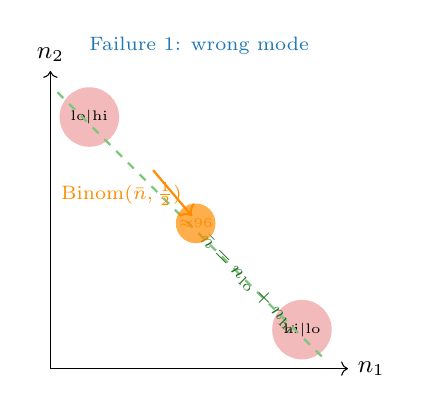
\begin{tikzpicture}[scale=0.9]
        \draw[->] (0,0) -- (4.2,0) node[right,font=\small]{$n_1$};
        \draw[->] (0,0) -- (0,4.2) node[above,font=\small]{$n_2$};
        \fill[slowred!40, opacity=0.8] (0.55,3.55) circle (0.42);
        \fill[slowred!40, opacity=0.8] (3.55,0.55) circle (0.42);
        \node[font=\tiny] at (0.55,3.55) {lo$|$hi};
        \node[font=\tiny] at (3.55,0.55) {hi$|$lo};
        \draw[coarsegreen!60,dashed,thick] (0.1,3.9) -- (3.9,0.1);
        \node[coarsegreen!70!black,font=\scriptsize,rotate=-45] at (2.8,1.2) {$\bar n = n_\text{lo}+n_\text{hi}$};
        \fill[intercolor,opacity=0.7] (2.05,2.05) circle (0.28);
        \draw[->,thick,intercolor] (1.45,2.8) -- (2.0,2.15)
          node[above left,font=\scriptsize,intercolor]{Binom$(\bar n,\tfrac12)$};
        \node[font=\tiny,intercolor] at (2.05,2.05) {$\approx$96};
        \node[above,font=\scriptsize,myblue] at (2.1, 4.3) {Failure 1: wrong mode};
      \end{tikzpicture}
      \end{center}

      \medskip
      \begin{center}
      \renewcommand{\arraystretch}{1.2}
      {\footnotesize
      \begin{tabular}{@{}ccc@{}}
        \toprule
        $k_{\rm rxn}$ & $\rho(n_A, n_B)$ & $P(\text{co-located})$ \\
        \midrule
        $0$ & $0.00$ & $76.6\%$ \emph{(Binom)} \\
        $5$ & $-0.80$ & $36.4\%$ \\
        $50$ & $-0.98$ & $\mathbf{4.0\%}$ \\
        \bottomrule
      \end{tabular}
      }
      \end{center}
      {\scriptsize Failure 2: independence assumption inflates co-location.}
    \end{column}
  \end{columns}

\end{frame}


% ================================================================
%  9. NEW (moved up): PatchQSD — the fix
% ================================================================
\begin{frame}{The patch QSD: physics-informed prolongation}

  \begin{columns}[T]
    \begin{column}{0.52\textwidth}

      \textbf{One unified fix for both failure modes.}

      \medskip
      Replace Binomial with the \textbf{quasi-stationary distribution (QSD)}
      of the local patch dynamics:
      \[
        \pi(n_1,\ldots,n_M \mid \bar{\mathbf{n}})
        = \text{QSD of } M\text{-voxel local CME}
      \]
      \vspace{-0.3em}
      where the local CME includes internal diffusion \emph{and} reactions
      within the patch, with reactions that leave the $\bar{\mathbf{n}}$ subspace
      treated as \textbf{absorbing} (QSD conditioning).

      \medskip
      \begin{block}{Generality}
        \textbf{M=2} (1D pair) $\cdot$ \textbf{M=4} (2D 2$\times$2) $\cdot$
        \textbf{M=8} (3D 2$\times$2$\times$2).\\
        Works for any \texttt{CoarseningMap} topology.\\
        Precomputed once: one small eigenproblem per $(\bar n_A, \bar n_B)$.
      \end{block}

      \medskip
      \begin{block}{Exact limits}
        $k_{\rm rxn}{=}0$, $d{\to}\infty$: QSD $\to$ Binom/Multinomial (recovers birth-death result exactly).\\[0.2em]
        Bistable propensities: QSD $\to$ bimodal (mass at both stable fixed points).\\[0.2em]
        Strong A+B${\to}\emptyset$: QSD captures A-B anti-correlation.
      \end{block}

    \end{column}
    \begin{column}{0.44\textwidth}

      \textbf{QSD vs Binomial at the bimolecular front}\\
      ($d{=}2$, $\bar n_A{=}\bar n_B{=}3$, varying $k_{\rm rxn}$):

      \medskip
      \begin{center}
      \renewcommand{\arraystretch}{1.35}
      \begin{tabular}{@{}ccc@{}}
        \toprule
        $k_{\rm rxn}$ & $\rho(n_{A,1},n_{B,1})$ & $P({\rm co-located})$ \\
        \midrule
        $0$   & $+0.000$ & $76.6\%$ \\
        \rowcolor{myblue!10}
        $0.5$ & $-0.095$ & $75.7\%$ \\
        $5$   & $-0.796$ & $36.4\%$ \\
        \rowcolor{slowred!10}
        $50$  & $-0.982$ & $\mathbf{4.0\%}$ \\
        \bottomrule
      \end{tabular}
      \end{center}

      \medskip
      {\footnotesize
        Binomial: always $76.6\%$ (independent assumption).\\[0.4em]
        QSD corrects the ${\sim}19\times$ overestimate at strong $k_{\rm rxn}$
        --- \emph{without any additional runtime cost}
        beyond the precomputed table.\\[0.4em]
        For covered states, the \textbf{multiplicative update}
        $p^{\rm new}(x) = \tilde p(x)\cdot\bar p^{\rm post}/\bar p^{\rm pre}$
        preserves the fine-level distribution exactly (no QSD approximation needed).
        QSD is used only for newly-added expand!\ states.
      }
    \end{column}
  \end{columns}

\end{frame}


% ================================================================
%  9. V-cycle + conditional prolongation (merged)
% ================================================================
\begin{frame}{The V-cycle with conditional prolongation}

\begin{columns}[T]
\column{0.46\textwidth}

\textbf{One V-cycle step:}\\[0.3em]
\begin{enumerate}\setlength\itemsep{0.22em}
  \item \textbf{Pre-smooth}: intra-pair diffusion for $\tau_{\rm pre}$
  \item \textbf{Restrict}: $\bar n_j = n_{2j-1}+n_{2j}$
  \item \textbf{Recurse}: V-cycle on $K/2$ voxels
  \item \textbf{Prolong}: conditional reconstruction
  \item \textbf{Prune}: remove states with $p(x) < \tau$
\end{enumerate}

\medskip
\textbf{Prolongation strategy:}

\textbf{Covered states} $(\bar x \in \calR\tilde p)$: multiplicative update
\[
  p^{\rm new}(x) = \tilde p(x)\cdot\frac{\bar p^{\rm post}(\bar x)}{\bar p^{\rm pre}(\bar x)}
\]
Asymmetry-preserving: mass at $(n_{\rm lo},n_{\rm hi})$ stays there.

\textbf{New states} (expand!-added):
use \textbf{patch QSD} $\pi(\bar n)$ --- the within-patch conditional (details next).

\column{0.50\textwidth}
\vspace{0.4em}
\begin{block}{Why not reconstruct at every step?}
  Forcing a Binomial split on every pair, every step, erases the
  within-pair asymmetry (the bistable front).\\[0.3em]
  Instead: evolve $p^h$ directly.
  Coarsening is \emph{only} for the recursive correction;
  the fine window tracks the true distribution exactly.
\end{block}

\vspace{0.4em}
\begin{alertblock}{Diffusion boundary states ($L_1{=}2$)}
  Coarse diffusion $({\bar n}_1,{\bar n}_2)\!\to\!({\bar n}_1{-}1,{\bar n}_2{+}1)$
  is always $L_1{=}2$.
  Without this neighbor search, \textbf{inter-pair mass transport is invisible}
  to the V-cycle and molecules never leave pair~1.
\end{alertblock}

\end{columns}

\end{frame}


% ================================================================
%  10. Schlögl wavefront result
% ================================================================
\begin{frame}{Result: Schl\"{o}gl wavefront spreading via the V-cycle}
\begin{center}
  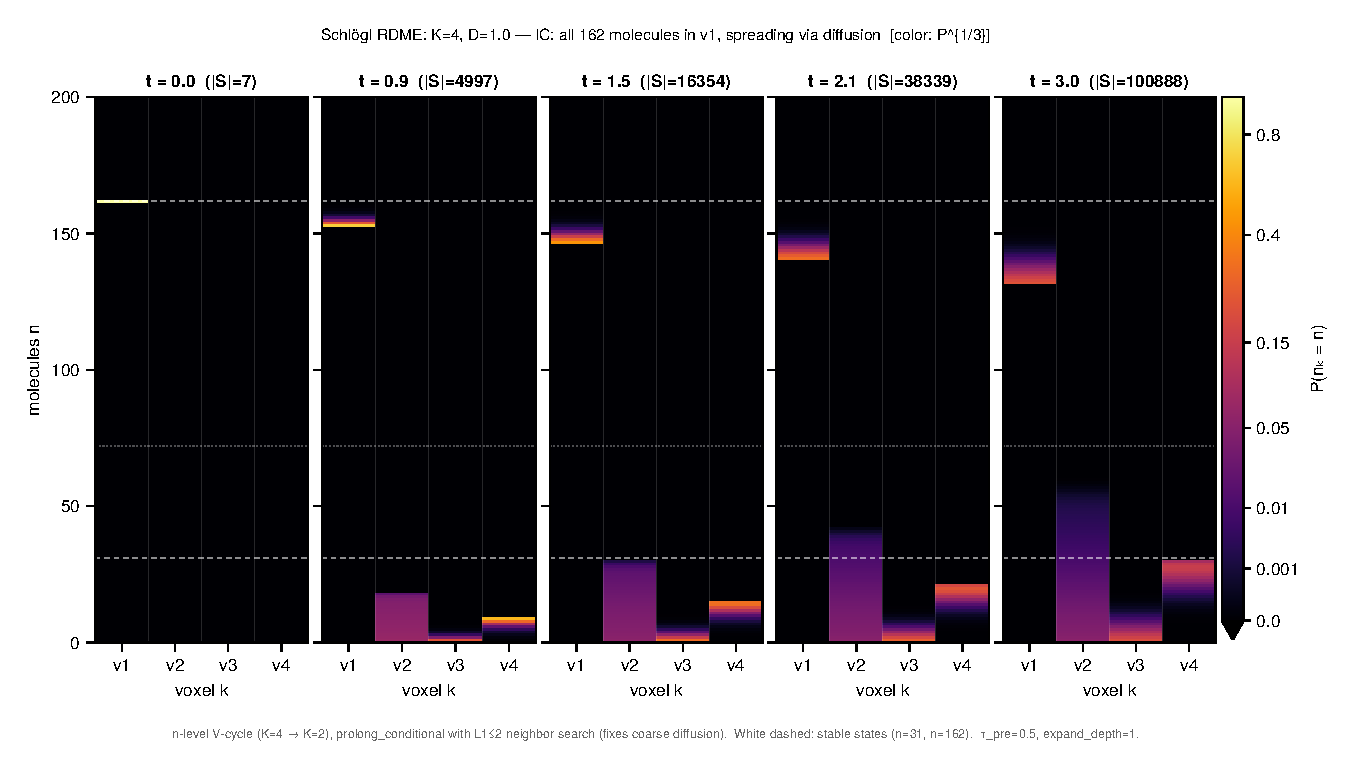
\includegraphics[width=0.93\textwidth,keepaspectratio]{fig_schlogl_wavefront}
\end{center}
\vspace{-0.5em}
{\footnotesize
$K{=}4$, $D{=}1.0$, IC: all $n_{\rm hi}{=}162$ molecules in $v_1$.
Conditional prolongation with $L_1{\leq}2$ neighbor search propagates mass from pair~1 to pair~2.
State space: $|S|{=}7 \to 100{,}888$ over $t{=}0 \to 3$ (controlled growth; no explosion).
White dashed: stable states ($n{=}31$, $n{=}162$). White dotted: unstable point ($n{=}72$).
}
\end{frame}


% ================================================================
%  11. NEW: A+B → ∅  2D front
% ================================================================
\begin{frame}{Two-species A+B$\to\emptyset$: mixed-resolution reaction front}
\begin{center}
  \includegraphics[width=0.94\textwidth,keepaspectratio]{mixed_annihilation_2d}
\end{center}
\vspace{-0.5em}
{\footnotesize
\textbf{Top row:} A (red) produced in top-left corner, B (blue) in bottom-right.
They diffuse toward the center and annihilate; \textbf{purple} = reaction zone (both species present).
White outline = active FSP strip (tracked stochastically); rest is exact mean-field.\\[0.2em]
\textbf{Bottom right (scaling):}
Full 2D FSP hits memory wall at $K{\approx}3$.
\textbf{Column-product} (independent 1D FSPs per active column, green): tractable for any $K$.
}
\end{frame}


% ================================================================
%  14. Summary
% ================================================================
\begin{frame}{Summary}

  \begin{block}{1.\quad Restriction + prolongation compresses the RDME state space.}
    When the within-patch distribution is near-Binomial/Multinomial,
    marginalizing patches reduces the state space from $n_{\max}^{2S}$ to $n_{\max}^{S}$ per patch.
    \emph{K=8 birth-death wavefront solved with 30k states (direct: intractable).}
  \end{block}

  \smallskip
  \begin{block}{2.\quad Conditional prolongation handles bistable and bimolecular fronts.}
    Multiplicative update for covered states preserves within-pair asymmetry.
    $L_1{\leq}2$ neighbor search propagates both reaction and diffusion boundaries.
    \emph{Schl\"{o}gl wavefront and bistable splitting correctly captured.}
  \end{block}

  \smallskip
  \begin{block}{3.\quad Mixed-resolution active set: the wavefront is always narrow.}
    Mean-field for inactive voxels (exact for linear reactions; QSD closure for bimolecular).
    Adaptive promote/demote keeps $K_{\rm act} = O(1)$ regardless of $K$.
    \emph{A+B$\to\emptyset$ reaction front tracked in 2D; column-product gives linear scaling in $K_y$.}
  \end{block}

  \smallskip
  \begin{block}{4.\quad Patch QSD: physics-informed prolongation for bimolecular reactions.}
    Generalizes Binomial ($M{=}2$) to arbitrary $M$-voxel neighborhoods.
    Captures A-B anti-correlation; corrects ${\sim}19\times$ overestimate of
    co-location probability under strong reactions.
    \emph{Precomputed once; plug-in replacement for Binomial/Multinomial.}
  \end{block}

\end{frame}


% ================================================================
%  Appendix
% ================================================================
\appendix


\begin{frame}{Appendix: Schl\"{o}gl splitting from the unstable fixed point}
\begin{center}
  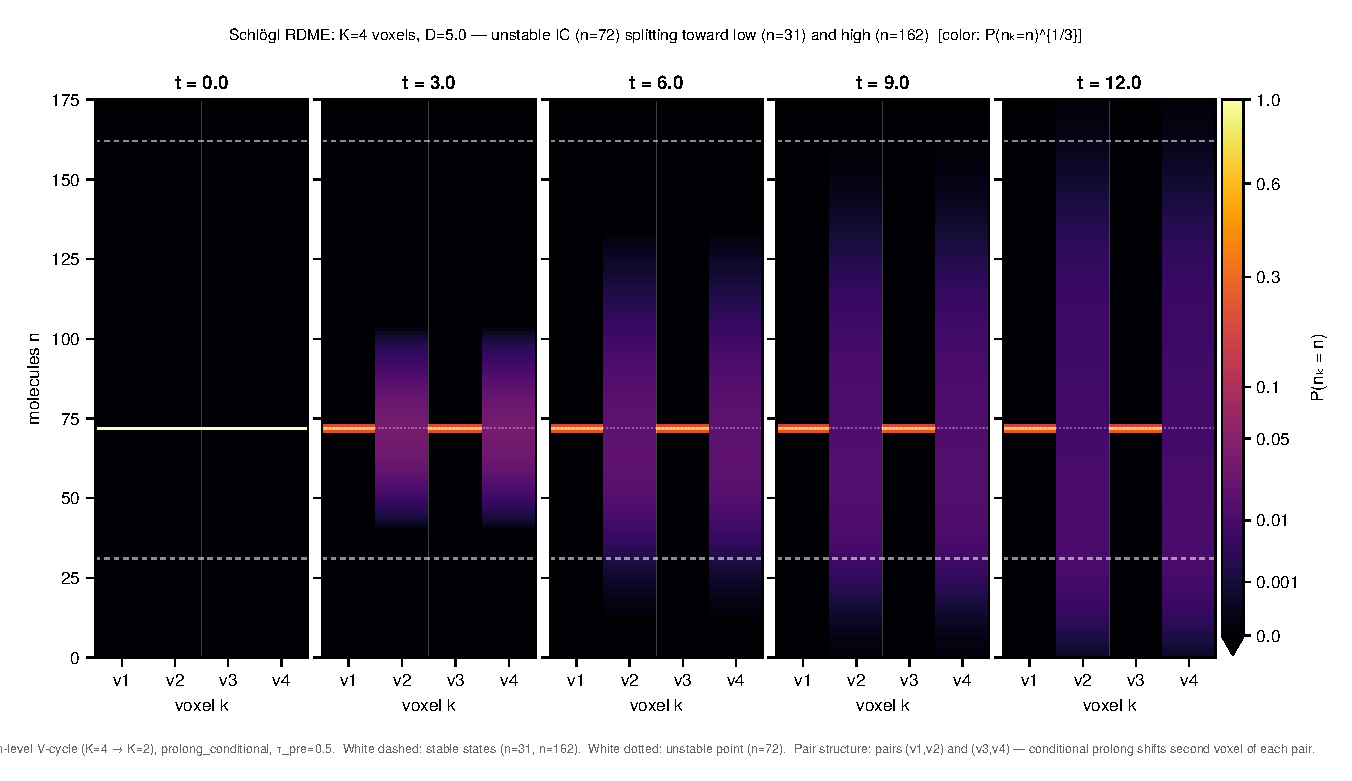
\includegraphics[width=0.93\textwidth,keepaspectratio]{fig_schlogl_splitting}
\end{center}
\vspace{-0.5em}
{\footnotesize
$K{=}4$, $D{=}5.0$, IC: all voxels at unstable point $n{=}72$.
By $t{=}12$: 37\% probability in low basin ($n{<}51$), 10\% entering high basin ($n{>}117$).
Color: $P(n_k{=}n)^{1/3}$ (cube-root scale to reveal low-probability tails).
}
\end{frame}

\begin{frame}{Appendix: mixed-resolution generator self-consistency}
  \begin{center}
    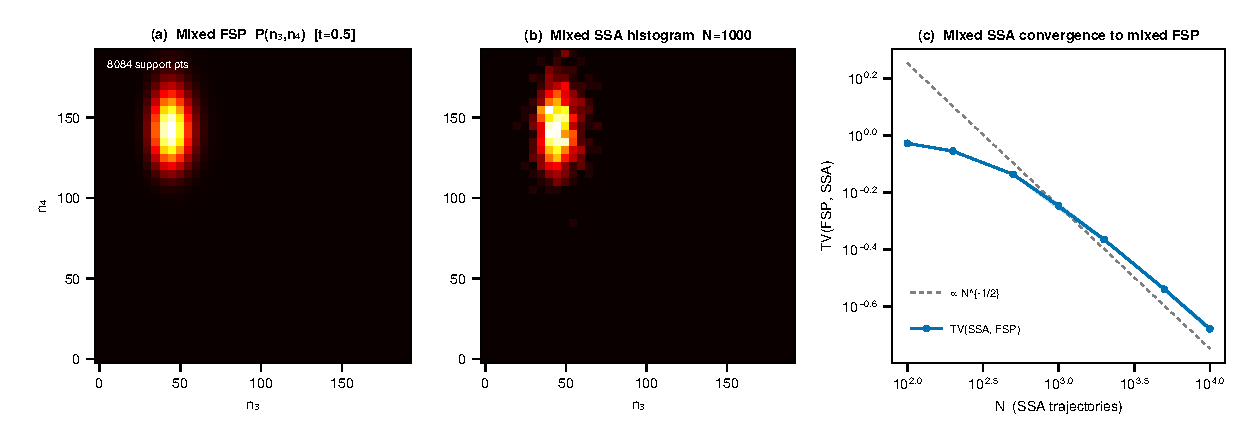
\includegraphics[width=0.78\textwidth,keepaspectratio]{fig_mixed_fsp_ssa}
  \end{center}
  {\footnotesize
    ODE solve on the mixed state $(\bar n_1, n_3, n_4)$
    vs.\ Monte Carlo on the same reduced generator.
    Means agree to ${<}1\%$; TV $\sim N^{-1/2}$ (sampling noise only).
  }
\end{frame}

\begin{frame}{Appendix: probability dynamics (birth-death vs.\ Schl\"{o}gl)}
\begin{center}
  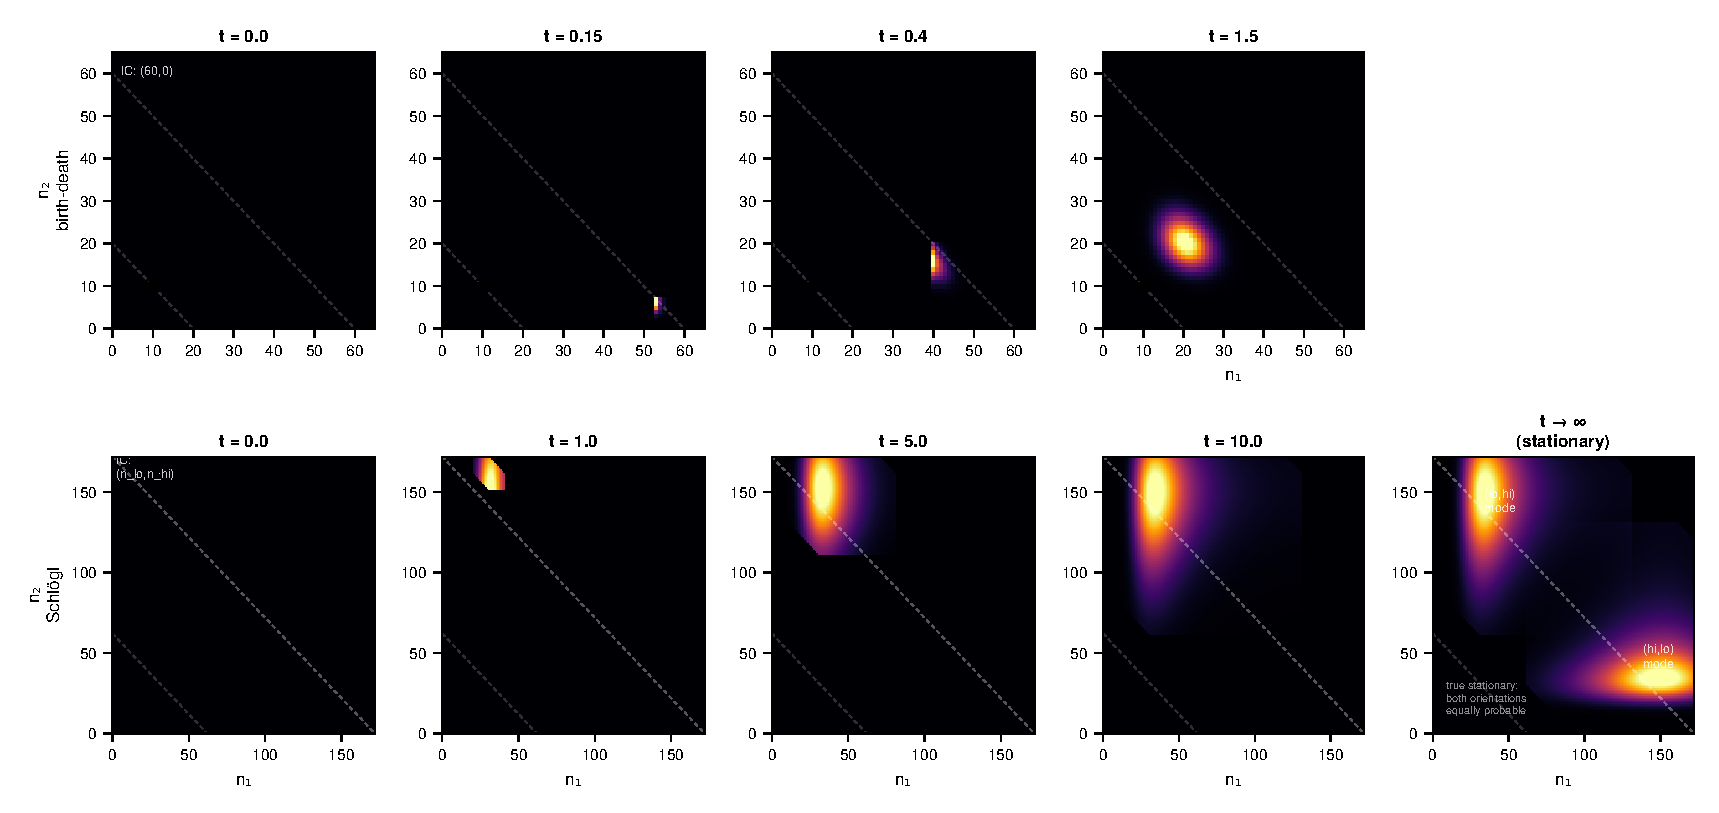
\includegraphics[width=0.92\textwidth,keepaspectratio]{fig_talk_diffusion}
\end{center}
{\footnotesize
\textbf{Top:} birth-death point source traveling to Poisson(10) stationary. Binomial coarsening exact.\\
\textbf{Bottom:} Schl\"{o}gl front IC persisting metastably; true stationary (rightmost) shows both orientations equally.}
\end{frame}

\begin{frame}{Appendix: K=8 persistent front}
  \begin{center}
    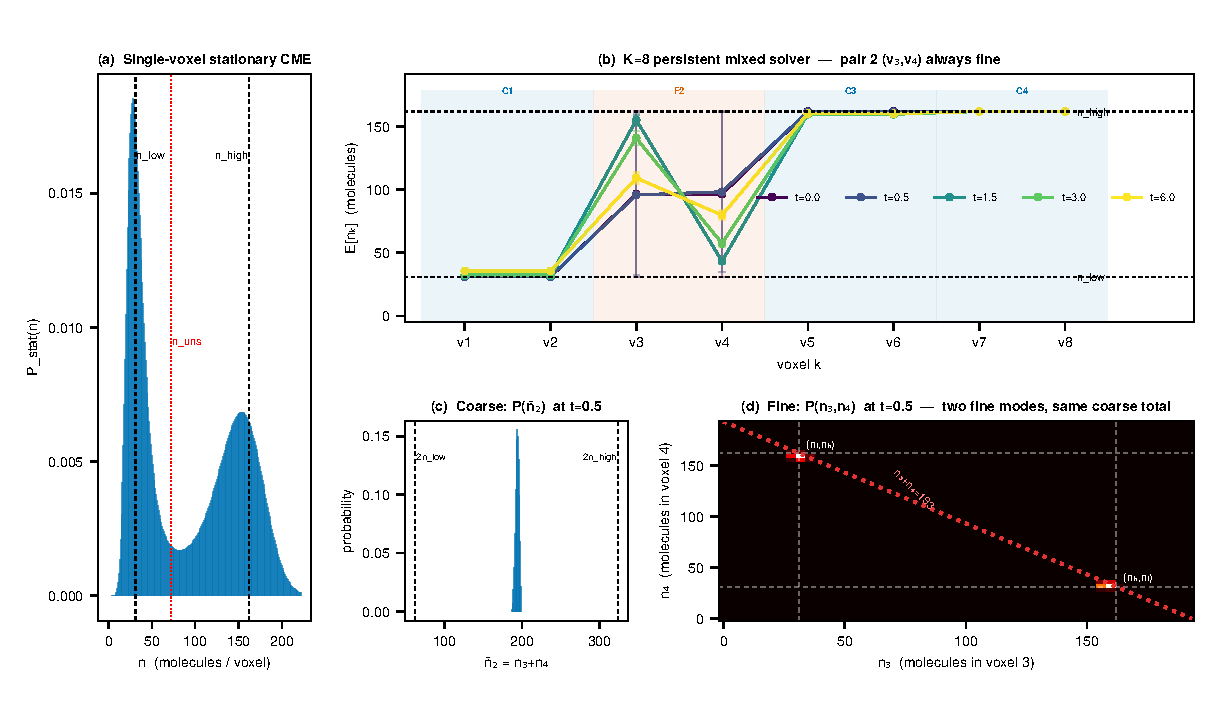
\includegraphics[width=0.82\textwidth,height=0.70\textheight,keepaspectratio]{fig_k8_persistent}
  \end{center}
\end{frame}

\end{document}
